\documentclass[tikz]{standalone}
\usepackage{amsmath}
\usetikzlibrary{decorations.pathreplacing}
\definecolor{bg}{HTML}{171D2B}
\definecolor{acc}{HTML}{F7B538}
\definecolor{blu}{HTML}{7DA9E8}
\definecolor{grn}{HTML}{7FD1A0}
\pagecolor{bg}
\begin{document}
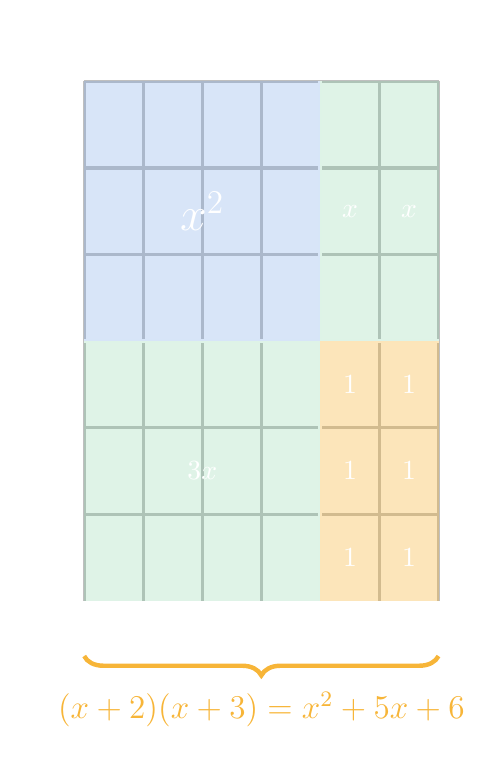
\begin{tikzpicture}[line width=1.2pt, scale=1.0]
  % dimensi: baris x = 3 baris (y 1.1..4.4), tiga baris satuan (y -2.2..1.1)
  % label kolom (atas)
  \node[white] at (1.5,4.85) {$x$};
  \node[white] at (3.375,4.85) {$2$};
  \node[white] at (4.125,4.85) {$2$};
  % label baris (kiri)
  \node[white] at (-0.5,2.75) {$x$};
  \node[white] at (-0.5,0.55) {$3$};
  \node[white] at (-0.5,-0.55) {$3$};
  \node[white] at (-0.5,-1.65) {$3$};
  % grid penuh
  \draw[gray!50] (0,-2.2) grid[xstep=0.75cm,ystep=1.1cm] (4.5,4.4);
  \draw[white, line width=1.4pt] (3,-2.2) -- (3,4.4);
  \draw[white, line width=1.4pt] (0,1.1) -- (4.5,1.1);
  % sel x^2 (biru): kolom x, baris x
  \fill[blu, opacity=0.30] (0,1.1) rectangle (3,4.4);
  \node[white, font=\LARGE] at (1.5,2.75) {$x^2$};
  % dua sel x (hijau): kolom satuan, baris x
  \fill[grn, opacity=0.25] (3,1.1) rectangle (4.5,4.4);
  \node[white] at (3.375,2.75) {$x$};
  \node[white] at (4.125,2.75) {$x$};
  % sel 3x (hijau): kolom x, baris satuan
  \fill[grn, opacity=0.25] (0,-2.2) rectangle (3,1.1);
  \node[white] at (1.5,-0.55) {$3x$};
  % enam kotak satuan (amber), masing-masing bernilai 1
  \fill[acc, opacity=0.35] (3,-2.2) rectangle (4.5,1.1);
  \node[white] at (3.375,0.55) {$1$};
  \node[white] at (4.125,0.55) {$1$};
  \node[white] at (3.375,-0.55) {$1$};
  \node[white] at (4.125,-0.55) {$1$};
  \node[white] at (3.375,-1.65) {$1$};
  \node[white] at (4.125,-1.65) {$1$};
  % kurung hasil
  \draw[acc, line width=1.6pt, decorate, decoration={brace, amplitude=7pt, mirror}]
    (0,-2.9) -- (4.5,-2.9)
    node[midway, below=9pt, acc, font=\large]{$(x+2)(x+3) = x^2 + 5x + 6$};
\end{tikzpicture}
\end{document}
